\documentclass[10pt]{article}
% Shared preamble for the course handouts and the cheatsheet (article class).
\usepackage[T1]{fontenc}
\usepackage[utf8]{inputenc}
\usepackage{lmodern}
\usepackage[a4paper, margin=2cm]{geometry}
\usepackage{amsmath, amssymb, bm, booktabs, graphicx, xcolor, enumitem, tcolorbox, multicol, listings}
\usepackage{tikz}
\usetikzlibrary{arrows.meta, positioning, calc}
\usepackage[hidelinks]{hyperref}
\setlength{\parindent}{0pt}
\setlength{\parskip}{0.5em}

% same colours and macros as the slides (slides/preamble.tex)
\definecolor{accent}{HTML}{C0392B}
\definecolor{cool}{HTML}{2E6DB4}
\definecolor{muted}{HTML}{7A7A7A}
\definecolor{good}{HTML}{2E8B57}
\definecolor{prob}{HTML}{E67E22}
\newcommand{\given}{\,|\,}
\newcommand{\E}{\mathbb{E}}
\newcommand{\KL}[2]{D_{\mathrm{KL}}\!\left[#1\,\middle\|\,#2\right]}
\newcommand{\N}{\mathcal{N}}
\newcommand{\Hess}{\mathcal{H}}
\DeclareMathOperator*{\argmin}{arg\,min}

% boxes
\newtcolorbox{keyidea}{colback=accent!5, colframe=accent!70!black, boxrule=0.6pt, arc=2pt, left=6pt, right=6pt, top=4pt, bottom=4pt}
\newtcolorbox{labhelp}[1]{colback=good!5, colframe=good!60!black, boxrule=0.6pt, arc=2pt, title={\small\bfseries #1}, fonttitle=\small, left=6pt, right=6pt, top=4pt, bottom=4pt}
\newtcolorbox{backupbox}[1]{colback=cool!5, colframe=cool!70!black, boxrule=0.6pt, arc=2pt, title={\small\bfseries #1}, left=6pt, right=6pt, top=4pt, bottom=4pt}

\lstset{basicstyle=\ttfamily\small, columns=fullflexible, keepspaces=true, showstringspaces=false,
  commentstyle=\color{muted}, keywordstyle=\color{cool}\bfseries, language=Python, frame=none,
  backgroundcolor=\color{black!3}, xleftmargin=4pt, aboveskip=4pt, belowskip=4pt}

\geometry{margin=1.4cm}
\setlength{\parskip}{0.3em}
\pagestyle{empty}

\begin{document}

{\Large\bfseries A robot that acts to know \;---\; cheatsheet}\hfill{\small\color{muted} keep it next to you all week}

\vspace{0.3em}
\section*{1. numpy: a distribution is an array}

\textbf{One axis per variable.} A belief over a discrete variable is a 1-D array that adds to 1.
A joint over two variables is a 2-D array: the first index is the first variable.
\begin{lstlisting}
p_S = np.array([0.3, 0.7])            # p(S): [open, closed]
p_O_given_S = np.array([[0.9, 0.1],   # row s: p(O | S = s)
                        [0.2, 0.8]])  # each ROW adds to 1
\end{lstlisting}

\textbf{Shapes.} \texttt{x.shape} tells you the axes. Print it whenever in doubt.
\begin{lstlisting}
p_S.shape            # (2,)
p_O_given_S.shape    # (2, 2)   axes [s, o]
\end{lstlisting}

\textbf{Adding an axis: \texttt{None}.} \texttt{x[:, None]} turns a vector of shape \texttt{(2,)}
into a column \texttt{(2, 1)}; \texttt{x[None, :]} into a row \texttt{(1, 2)}.

\textbf{Broadcasting.} When two arrays are combined, numpy compares their shapes from the
right. An axis of size 1 is \emph{stretched} to match the other array. So a column times a
matrix multiplies every column of the matrix by the column vector:
\begin{lstlisting}
joint = p_O_given_S * p_S[:, None]
#        (2, 2)       (2, 1) -> stretched to (2, 2)
# joint[s, o] = p(o | s) p(s)     the product rule
\end{lstlisting}
Without \texttt{[:, None]}, \texttt{p\_S} would be read as a \emph{row} and multiply the
wrong axis, silently. Always line the axes up yourself.

\begin{center}
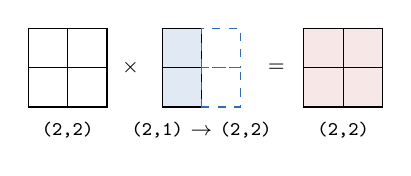
\begin{tikzpicture}[x=0.5cm, y=0.5cm, font=\scriptsize]
  \foreach \i in {0,1} \foreach \j in {0,1} \draw (\j,-\i) rectangle ++(1,1);
  \node at (1,-1.6) {\texttt{(2,2)}};
  \node at (2.6,0) {$\times$};
  \foreach \i in {0,1} \draw[fill=cool!15] (3.4,-\i) rectangle ++(1,1);
  \foreach \i in {0,1} \draw[dashed, cool] (4.4,-\i) rectangle ++(1,1);
  \node at (4.4,-1.6) {\texttt{(2,1)} $\to$ \texttt{(2,2)}};
  \node at (6.3,0) {$=$};
  \foreach \i in {0,1} \foreach \j in {0,1} \draw[fill=accent!12] (7+\j,-\i) rectangle ++(1,1);
  \node at (8,-1.6) {\texttt{(2,2)}};
\end{tikzpicture}
\end{center}

\textbf{Three variables.} Give each its own axis and pad with \texttt{None} where a
factor does not depend on that variable:
\begin{lstlisting}
# joint[s, a, o] = p(s) p(a) p(o | s, a)
j = p_S[:, None, None] * p_A[None, :, None] * p_O_given_SA
#    (2,1,1)              (1,2,1)              (2,2,2)
\end{lstlisting}

\textbf{Marginalise = sum over an axis.} The summed axis disappears.
\begin{lstlisting}
p_O  = joint.sum(axis=0)       # sum over s -> p(O), shape (2,)
p_SA = j.sum(axis=2)           # sum over o -> p(S, A)
p_A  = j.sum(axis=(0, 2))      # sum over s and o
\end{lstlisting}
The notebook reorders the axes to \texttt{[s, o, a]} with \texttt{j.transpose(0, 2, 1)}: then
\texttt{sum(axis=(0, 2))} gives $p(O)$. Always check which axis is which variable.

\textbf{Condition = take a slice, divide by its sum.}
\begin{lstlisting}
col = joint[:, 0]              # o = gap: shape (2,)
p_S_given_gap = col / col.sum()        # = col / p_O[0]
p_S_given_O = joint / p_O[None, :]     # every column at once
\end{lstlisting}
\texttt{keepdims=True} keeps the summed axis with size 1, so it broadcasts back:
\texttt{joint / joint.sum(axis=0, keepdims=True)}.

\textbf{Checks that save an hour.}
\begin{lstlisting}
joint.sum()                    # 1.0 ?
np.allclose(a, b)              # equal up to rounding
p_S_given_O.sum(axis=0)        # each column adds to 1 ?
\end{lstlisting}

\textbf{Densities on a grid.} A continuous belief becomes values on a grid of points;
integrals become sums times the spacing.
\begin{lstlisting}
s  = np.linspace(0.0, 4.0, 2001); ds = s[1] - s[0]
p  = np.exp(-0.5*(s - 2)**2/0.25) / np.sqrt(2*np.pi*0.25)
p.sum() * ds                   # ~ 1: the integral
(s * p).sum() * ds             # the mean, E[s]
\end{lstlisting}

\textbf{Sampling.} \texttt{rng = np.random.default\_rng(0)}; \texttt{rng.normal(mu, sd, n)};
\texttt{rng.random(n) < p} is \texttt{True} with probability \texttt{p};
\texttt{np.where(cond, a, b)} picks \texttt{a} where \texttt{cond} holds, else \texttt{b}.
Boolean masks select: \texttt{x[mask].mean()}.

\newpage

\section*{2. The three operations}
\renewcommand{\arraystretch}{1.5}
\begin{tabular}{@{}ll@{}}
factorise & $p(s,o) = p(o\given s)\,p(s)$ \\
marginalise & $p(o) = \sum_s p(s,o)$ \;or\; $\int p(s,o)\,ds$ \\
condition & $p(s\given o) = p(s,o)/p(o)$ \\
Bayes & $p(s\given o) = \dfrac{p(o\given s)\,p(s)}{p(o)}$ \\
\end{tabular}

\textbf{Names.} $p(s)$ prior;\; $p(o\given s)$ likelihood (sensor model);\;
$p(o)$ evidence;\; $p(s\given o)$ posterior;\; $q(s)$ the robot's belief.
Time: $s_t$ at step $t$;\; $o_{<t}$ all readings before $t$;\; $o_{\le t}$ up to $t$;\;
$a_t$ the action at step $t$.

\section*{3. Gaussians}
\[
\N(x;\mu,\sigma^2) = \frac{1}{\sqrt{2\pi\sigma^2}}\,e^{-\frac{(x-\mu)^2}{2\sigma^2}},
\qquad -\ln\N = \frac{(x-\mu)^2}{2\sigma^2} + \tfrac12\ln(2\pi\sigma^2)
\]
\textbf{Precision} $\pi = 1/\sigma^2$: how sure. $\pm\sigma$ holds 68\%, $\pm2\sigma$ 95\%.

\textbf{Two Gaussians multiplied} (prior $\times$ reading): precisions add, means average by precision
\[
\pi = \pi_p + \pi_o, \qquad \mu = \frac{\pi_p m + \pi_o o}{\pi_p + \pi_o}.
\]
\textbf{Conditioning a 2-D Gaussian} on a reading $o^*$ (gain form):
$k = \Sigma_{so}/\Sigma_{oo}$,\; $\mu_{s\mid o} = \mu_s + k\,(o^* - \mu_o)$,\; $\Sigma_{s\mid o} = \Sigma_{ss} - k\,\Sigma_{so}$.

\textbf{Kalman step} (move $a$, then read $o$): $\mu_- = \mu - a$, $\sigma_-^2 = \sigma^2 + \sigma_w^2$;\;
$k = \sigma_-^2/(\sigma_-^2+\sigma_v^2)$, $\mu \leftarrow \mu_- + k(o-\mu_-)$, $\sigma^2 \leftarrow (1-k)\sigma_-^2$.

\textbf{Entropy} of a Gaussian: $\tfrac12\ln(2\pi e\,\sigma^2)$.\;
\textbf{KL} $\KL{\N(\mu_1,\sigma_1^2)}{\N(\mu_0,\sigma_0^2)} = \ln\frac{\sigma_0}{\sigma_1} + \frac{\sigma_1^2 + (\mu_1-\mu_0)^2}{2\sigma_0^2} - \frac12$.

\section*{4. Logs, averages, information}
$\ln(ab) = \ln a + \ln b$;\; $\ln(a/b) = \ln a - \ln b$;\; $\ln e^x = x$;\; $\ln 1 = 0$.\\
$-\ln p$: a cost in \textbf{nats}; rare readings cost more.\\
Expectation: $\E_q[f] = \int q(s)\,f(s)\,ds$ (a sum for discrete $s$): one number.\\
$\E_q[c] = c$ for a constant;\; $\int q = 1$;\; $\E_q[s-\mu] = 0$,\; $\E_q[(s-\mu)^2] = \sigma^2$.\\
KL: $\KL{q}{p} = \E_q[\ln q - \ln p] \ge 0$, zero only when $q = p$.

\section*{5. Derivatives}
$\frac{d}{dx}x^2 = 2x$;\; $\frac{d}{dx}\ln x = 1/x$;\; $\frac{d}{dx}e^{x} = e^{x}$;\;
$\frac{d}{dx}(x-c)^2 = 2(x-c)$.\\
\textbf{Chain rule:} $\frac{d}{dx}f(g(x)) = f'(g(x))\,g'(x)$.\;
\textbf{Partial} $\partial F/\partial x$: the slope in $x$ with every other variable held fixed.\\
\textbf{Taylor} around $\mu$: $f(s) \approx f(\mu) + f'(\mu)(s-\mu) + \tfrac12 f''(\mu)(s-\mu)^2$;\;
$f''$ is the \textbf{curvature} (Hessian $\Hess$ in several variables).\\
\textbf{Minimum:} slope $= 0$ and curvature $> 0$.\;
\textbf{Gradient step:} $x \leftarrow x - \eta\,\partial F/\partial x$, with a small step size $\eta$;
for a parabola of curvature $\Hess$ it converges when $\eta < 2/\Hess$.

\section*{6. The free energy, in one box}
\begin{keyidea}\small
$F[q,o] = \E_q[\ln q(s) - \ln p(o,s)] = \KL{q}{p(s\given o)} - \ln p(o) \ge -\ln p(o)$\\[2pt]
$\phantom{F[q,o]} = \KL{q(s)}{p(s)} - \E_q[\ln p(o\given s)]$ \;(complexity $-$ accuracy)\\[2pt]
Laplace, $q = \N(\mu,\sigma^2)$: $F \approx -\ln p(o,\mu) + \tfrac12\Hess\sigma^2 - \tfrac12\ln(2\pi e\sigma^2)$, best $\sigma^2 = 1/\Hess$.
\end{keyidea}

\end{document}
